% Options for packages loaded elsewhere
\PassOptionsToPackage{unicode}{hyperref}
\PassOptionsToPackage{hyphens}{url}
\PassOptionsToPackage{dvipsnames,svgnames,x11names}{xcolor}
%
\documentclass[
  letterpaper,
  DIV=11,
  numbers=noendperiod]{scrartcl}

\usepackage{amsmath,amssymb}
\usepackage{iftex}
\ifPDFTeX
  \usepackage[T1]{fontenc}
  \usepackage[utf8]{inputenc}
  \usepackage{textcomp} % provide euro and other symbols
\else % if luatex or xetex
  \usepackage{unicode-math}
  \defaultfontfeatures{Scale=MatchLowercase}
  \defaultfontfeatures[\rmfamily]{Ligatures=TeX,Scale=1}
\fi
\usepackage{lmodern}
\ifPDFTeX\else  
    % xetex/luatex font selection
\fi
% Use upquote if available, for straight quotes in verbatim environments
\IfFileExists{upquote.sty}{\usepackage{upquote}}{}
\IfFileExists{microtype.sty}{% use microtype if available
  \usepackage[]{microtype}
  \UseMicrotypeSet[protrusion]{basicmath} % disable protrusion for tt fonts
}{}
\makeatletter
\@ifundefined{KOMAClassName}{% if non-KOMA class
  \IfFileExists{parskip.sty}{%
    \usepackage{parskip}
  }{% else
    \setlength{\parindent}{0pt}
    \setlength{\parskip}{6pt plus 2pt minus 1pt}}
}{% if KOMA class
  \KOMAoptions{parskip=half}}
\makeatother
\usepackage{xcolor}
\setlength{\emergencystretch}{3em} % prevent overfull lines
\setcounter{secnumdepth}{-\maxdimen} % remove section numbering
% Make \paragraph and \subparagraph free-standing
\makeatletter
\ifx\paragraph\undefined\else
  \let\oldparagraph\paragraph
  \renewcommand{\paragraph}{
    \@ifstar
      \xxxParagraphStar
      \xxxParagraphNoStar
  }
  \newcommand{\xxxParagraphStar}[1]{\oldparagraph*{#1}\mbox{}}
  \newcommand{\xxxParagraphNoStar}[1]{\oldparagraph{#1}\mbox{}}
\fi
\ifx\subparagraph\undefined\else
  \let\oldsubparagraph\subparagraph
  \renewcommand{\subparagraph}{
    \@ifstar
      \xxxSubParagraphStar
      \xxxSubParagraphNoStar
  }
  \newcommand{\xxxSubParagraphStar}[1]{\oldsubparagraph*{#1}\mbox{}}
  \newcommand{\xxxSubParagraphNoStar}[1]{\oldsubparagraph{#1}\mbox{}}
\fi
\makeatother


\providecommand{\tightlist}{%
  \setlength{\itemsep}{0pt}\setlength{\parskip}{0pt}}\usepackage{longtable,booktabs,array}
\usepackage{calc} % for calculating minipage widths
% Correct order of tables after \paragraph or \subparagraph
\usepackage{etoolbox}
\makeatletter
\patchcmd\longtable{\par}{\if@noskipsec\mbox{}\fi\par}{}{}
\makeatother
% Allow footnotes in longtable head/foot
\IfFileExists{footnotehyper.sty}{\usepackage{footnotehyper}}{\usepackage{footnote}}
\makesavenoteenv{longtable}
\usepackage{graphicx}
\makeatletter
\def\maxwidth{\ifdim\Gin@nat@width>\linewidth\linewidth\else\Gin@nat@width\fi}
\def\maxheight{\ifdim\Gin@nat@height>\textheight\textheight\else\Gin@nat@height\fi}
\makeatother
% Scale images if necessary, so that they will not overflow the page
% margins by default, and it is still possible to overwrite the defaults
% using explicit options in \includegraphics[width, height, ...]{}
\setkeys{Gin}{width=\maxwidth,height=\maxheight,keepaspectratio}
% Set default figure placement to htbp
\makeatletter
\def\fps@figure{htbp}
\makeatother
% definitions for citeproc citations
\NewDocumentCommand\citeproctext{}{}
\NewDocumentCommand\citeproc{mm}{%
  \begingroup\def\citeproctext{#2}\cite{#1}\endgroup}
\makeatletter
 % allow citations to break across lines
 \let\@cite@ofmt\@firstofone
 % avoid brackets around text for \cite:
 \def\@biblabel#1{}
 \def\@cite#1#2{{#1\if@tempswa , #2\fi}}
\makeatother
\newlength{\cslhangindent}
\setlength{\cslhangindent}{1.5em}
\newlength{\csllabelwidth}
\setlength{\csllabelwidth}{3em}
\newenvironment{CSLReferences}[2] % #1 hanging-indent, #2 entry-spacing
 {\begin{list}{}{%
  \setlength{\itemindent}{0pt}
  \setlength{\leftmargin}{0pt}
  \setlength{\parsep}{0pt}
  % turn on hanging indent if param 1 is 1
  \ifodd #1
   \setlength{\leftmargin}{\cslhangindent}
   \setlength{\itemindent}{-1\cslhangindent}
  \fi
  % set entry spacing
  \setlength{\itemsep}{#2\baselineskip}}}
 {\end{list}}
\usepackage{calc}
\newcommand{\CSLBlock}[1]{\hfill\break\parbox[t]{\linewidth}{\strut\ignorespaces#1\strut}}
\newcommand{\CSLLeftMargin}[1]{\parbox[t]{\csllabelwidth}{\strut#1\strut}}
\newcommand{\CSLRightInline}[1]{\parbox[t]{\linewidth - \csllabelwidth}{\strut#1\strut}}
\newcommand{\CSLIndent}[1]{\hspace{\cslhangindent}#1}

\KOMAoption{captions}{tableheading}
\makeatletter
\@ifpackageloaded{caption}{}{\usepackage{caption}}
\AtBeginDocument{%
\ifdefined\contentsname
  \renewcommand*\contentsname{Table of contents}
\else
  \newcommand\contentsname{Table of contents}
\fi
\ifdefined\listfigurename
  \renewcommand*\listfigurename{List of Figures}
\else
  \newcommand\listfigurename{List of Figures}
\fi
\ifdefined\listtablename
  \renewcommand*\listtablename{List of Tables}
\else
  \newcommand\listtablename{List of Tables}
\fi
\ifdefined\figurename
  \renewcommand*\figurename{Figure}
\else
  \newcommand\figurename{Figure}
\fi
\ifdefined\tablename
  \renewcommand*\tablename{Table}
\else
  \newcommand\tablename{Table}
\fi
}
\@ifpackageloaded{float}{}{\usepackage{float}}
\floatstyle{ruled}
\@ifundefined{c@chapter}{\newfloat{codelisting}{h}{lop}}{\newfloat{codelisting}{h}{lop}[chapter]}
\floatname{codelisting}{Listing}
\newcommand*\listoflistings{\listof{codelisting}{List of Listings}}
\makeatother
\makeatletter
\makeatother
\makeatletter
\@ifpackageloaded{caption}{}{\usepackage{caption}}
\@ifpackageloaded{subcaption}{}{\usepackage{subcaption}}
\makeatother

\ifLuaTeX
  \usepackage{selnolig}  % disable illegal ligatures
\fi
\usepackage{bookmark}

\IfFileExists{xurl.sty}{\usepackage{xurl}}{} % add URL line breaks if available
\urlstyle{same} % disable monospaced font for URLs
\hypersetup{
  pdftitle={Heat3d: A Study on 3D Heatmaps},
  pdfauthor={Tyler Wiederich},
  colorlinks=true,
  linkcolor={blue},
  filecolor={Maroon},
  citecolor={Blue},
  urlcolor={Blue},
  pdfcreator={LaTeX via pandoc}}


\title{Heat3d: A Study on 3D Heatmaps}
\author{Tyler Wiederich}
\date{April 28, 2025}

\begin{document}
\maketitle
\begin{abstract}
This is the abstact
\end{abstract}


\section{Introduction}\label{introduction}

\section{Literature Review}\label{literature-review}

\section{Methods}\label{methods}

Our study is designed to evaluate and expand the literature on numerical
estimation of 3D cha\texttt{heatmap3d} package in R, which allows for
the creation of 3D heatmaps with customizable parameters. The heatmaps
will be generated using a set of random data points, and we will vary
the number of data points, the color scheme, and the perspective of the
heatmap.rts. In our study, our focus is on 2D and 3D heatmaps, which we
\ldots{}

In this section, we discuss process of designing our experiment.

\subsection{Stimuli}\label{stimuli}

We denote ``stimuli'' to represent the magnitude of our chosen values.
In a 3D Cartesian space, the X- and Y- axes represent the coordinates of
the stimuli, and the stimuli lies on the Z-axis. For a 2D space, the
Z-axis is replaced by a color gradient scale. All stimuli and remaining
randomly generated values range between 0 and 100 units. In this
experiment, \(X=1, 2, \dots,10\) and \(Y=1, 2,\dots,10\).

(Lack of studies on what stimuli to choose)

The design of our experiment makes use of the method of constant
stimuli, where comparisons between stimuli are with respect to a stimuli
that remains the same magnitude (Kingdom and Prins 2016, chap. 3). We
set the constant stimuli at 50 units. For stimuli between 50 and 100, we
set the maximum stimuli magnitude at 90 and equally partitioned the
ratios with the constant stimuli, \(\frac{50}{90}=0.556\) to
\(\frac{50}{50}=1.0\), resulting in 4 varying stimuli values. The same
ratios obtained with stimuli between 50 and 90 were used to create
stimuli 4 varying between 0 and 50. Additionally, we also included a
stimuli pair where both values are 50, resulting in 9 total pairs of
stimuli. All stimuli values can be found in
\textbf{?@fig-stimuli-values}.

\begin{figure}[H]

{\centering 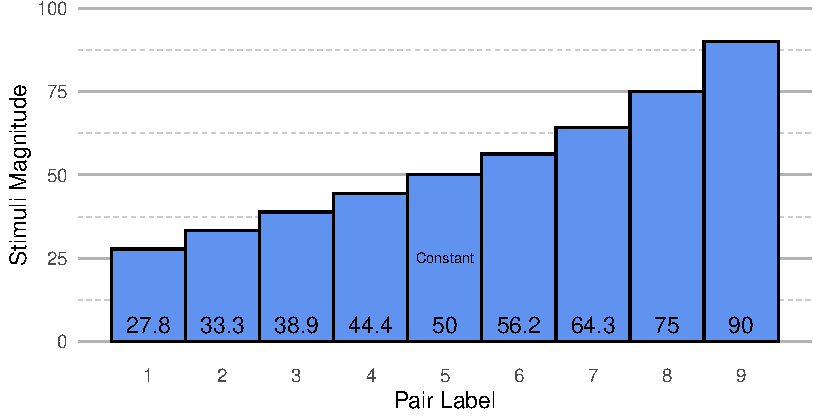
\includegraphics{index_files/figure-pdf/stimuli-values-1.pdf}

}

\caption{Caption}

\end{figure}%

To generate non-stimuli random values, we used a mixture distribution of
random uniform noise and a mathematical function. The mathematical
functions are scaled between 0 and 100,
\(g(Z)=100\cdot\frac{Z-\min(Z)}{\max(Z)-min(Z)}\). Two datasets were
created for the experiment. The first dataset, called set 1, used the
formula for the top half of sphere,
\(f_1(X,Y)=\sqrt{7^2-(X-\bar{X})^2-(Y-\bar{Y})^2}\). The second dataset
is calculated similarly using the formula for the bottom half of sphere,
\(f_2(X,Y)=\sqrt{7^2-(X-\bar{X})^2+(Y-\bar{Y})^2}\). Denoting \(Z\) as
the random values, \(U(0,100)\) as random variable drawn from a
continuous uniform distribution, and \(X,Y\) as heatmap coordinates, our
random heatmap data is calculated in Equation~\ref{eq-random-z} with
\(c=0.3\):

\begin{equation}\phantomsection\label{eq-random-z}{
Z=c\cdot U(0,100)+(1-c)\cdot g(f_i(X,Y))
}\end{equation}

\begin{figure}

\begin{minipage}{0.20\linewidth}

\centering{


\includegraphics{plots/z100.png}

}

\subcaption{\label{fig-z100}\(c=0\)}

\end{minipage}%
%
\begin{minipage}{0.20\linewidth}

\centering{

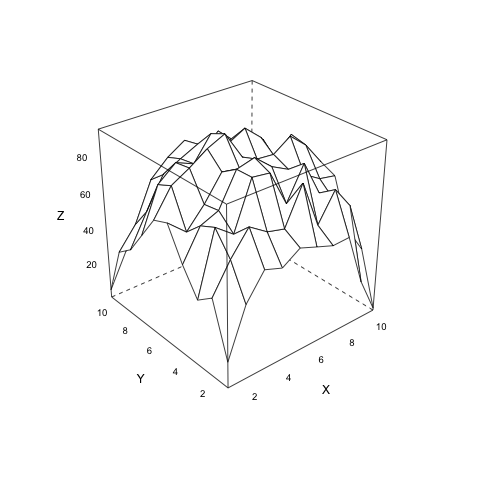
\includegraphics{plots/z75.png}

}

\subcaption{\label{fig-z75}\(c=0.25\)}

\end{minipage}%
%
\begin{minipage}{0.20\linewidth}

\centering{

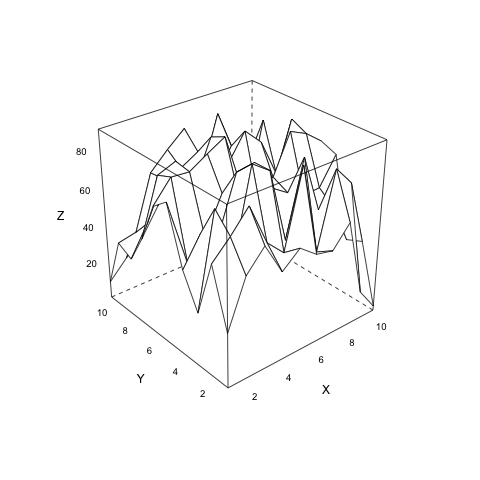
\includegraphics{plots/z50.png}

}

\subcaption{\label{fig-z50}\(c=0.5\)}

\end{minipage}%
%
\begin{minipage}{0.20\linewidth}

\centering{

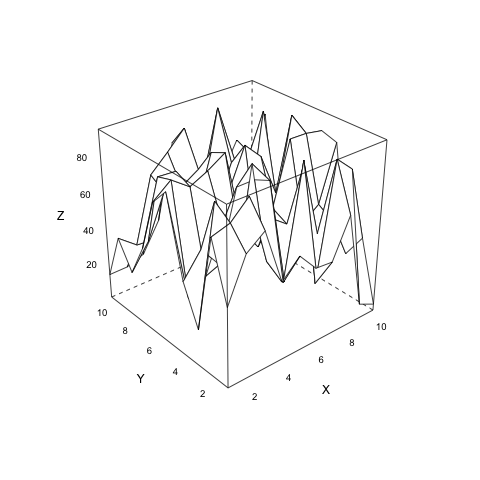
\includegraphics{plots/z25.png}

}

\subcaption{\label{fig-z25}\(c=0.75\)}

\end{minipage}%
%
\begin{minipage}{0.20\linewidth}

\centering{

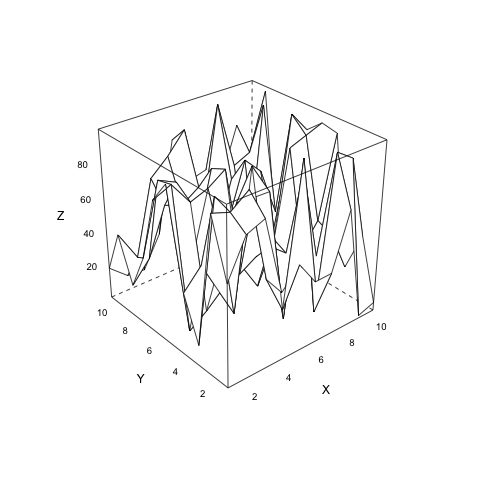
\includegraphics{plots/z0.png}

}

\subcaption{\label{fig-z0}\(c=1\)}

\end{minipage}%

\caption{\label{fig-random-z}Mixture distribution}

\end{figure}%

The placement of stimuli values onto the randomly generated heatmap data
was done via simulation to try to make their placement look as naturally
as possible. Twenty randomly heatmaps were generated. For each heatmap,
the non-constant stimuli was placed onto the coordinate such that the
difference between the stimuli and randomly generated value is
minimized. The constant stimuli was then placed onto a coordinate with a
Manhattan distance of 3 or 4 that minimizes the difference.

To ensure that stimuli placement is evenly position across the heatmap,
the count of stimuli was computed separately across the X and Y axes.
Chi-squared statistics were calculated for each axis and the heatmap
with the smallest average Chi-squared statistic was selected as the
final dataset.

\subsection{Charts}\label{charts}

Three types of charts are considered for this study: 2D-digital (2dd),
3D-digital (3dd), and 3D-printed (3dp). We constructed these charts so
that they are as similar as possible, but inherent difference between
dimensionality led to artistic decisions

The 3D-printed charts were rendered with OpenSCAD (XXX). To include plot
text, a 120mm by 120mm by 10mm base was created with a solid color.
Cells of the heatmap measured 10mm by 10mm, resulting in a heatmap that
is 100mm by 100mm. The maximum height of the heatmap values is 100mm.
Once rendered, the heatmap was saved to 3mf and stl files.

Solid and gradient filaments were used to print the OpenSCAD output
files\ldots{}

To closely match the 3D-digital chart to the 3D-printed chart, multiple
stl files were created for each colored component and combined with the
RGL package (XXX). The base was rendered with white smoke (\#F5F5F5) to
slightly contrast with the background color. Heatmap tiles were rendered
with cyan (\#74CCFF) and text labels were rendered with black
(\#000000). Lighting was placed at 45 degree angles at two opposite
corners of the chart.

Unlike the 3D charts, the 2D charts needed additional encodings to
convey heatmap values. The 2D heatmaps were created with ggplot2 using
geom\_tile. Fill colors for the cells use a color gradient from dark
blue (\#0C2841) to cyan (\#66D9FF), which were selected from a color
picker using shadows on our initial 3D-printed charts.

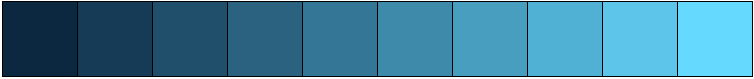
\includegraphics{index_files/figure-pdf/unnamed-chunk-3-1.pdf}

\begin{figure}[H]

{\centering \includegraphics{.pdf}

}

\caption{Picture of 3D printed chart}

\end{figure}%

\subsection{Experimental Design}\label{experimental-design}

\subsection{Subject Recruitment}\label{subject-recruitment}

\section*{Discussion}\label{discussion}
\addcontentsline{toc}{section}{Discussion}

\phantomsection\label{refs}
\begin{CSLReferences}{1}{0}
\bibitem[\citeproctext]{ref-kingdom2016}
Kingdom, Frederick A. A., and Nicolaas Prins. 2016. \emph{Psychophysics:
A Practical Introduction}. Second edition. Amsterdam: Elsevier/Academic
Press.

\end{CSLReferences}




\end{document}
